\section{The Sound of sequences}
La  On-line Encyclopedia of Integer Sequences (o OEIS) és una base de dades de seqüències de nombres trets de totes les branques d'investigació científica. Conté seqüències clàssiques com la llista de nombres primers o la seqüència amb els nombres de Fibonacci, o altres seqüències menys conegudes extretes de la resolució de problemes matemàtics, com ara el ``nombre de grafs planars amb n vèrtexs''. La base de dades la va començar l'any 1964 el matemàtic Neil J. A. Sloane com una eina per identificar i entendre seqüències. Avui inclou més de 300 000 seqüències.  

Les seqüències es poden analitzar matemàticament, visualitzant-les com a gràfiques de funció, o transformant-les en sons que es poden sentir, com en aquest cas. A més de revelar qualitats de la seqüència que no eren òbvies mirant els nombres, les peces de ``música'' són interessants a la seva manera. Esperem que n'escolteu algunes en aquest mòdul.  

Per transformar una seqüència a música, utilitzem un algorisme molt simple. Col·loquem la seqüència a les notes d'un piano. Aquest piano té 88 tecles i les numerem del zero fins al 87. Agafem els elements de la seqüència i hi sumem o hi restem múltiples de 88 fins que aconseguim un nombre dins del rang de 0 a 87. En termes tècnics, llegim la seqüència ``mòdul 88''.

\begin{figure}[h]
\centering
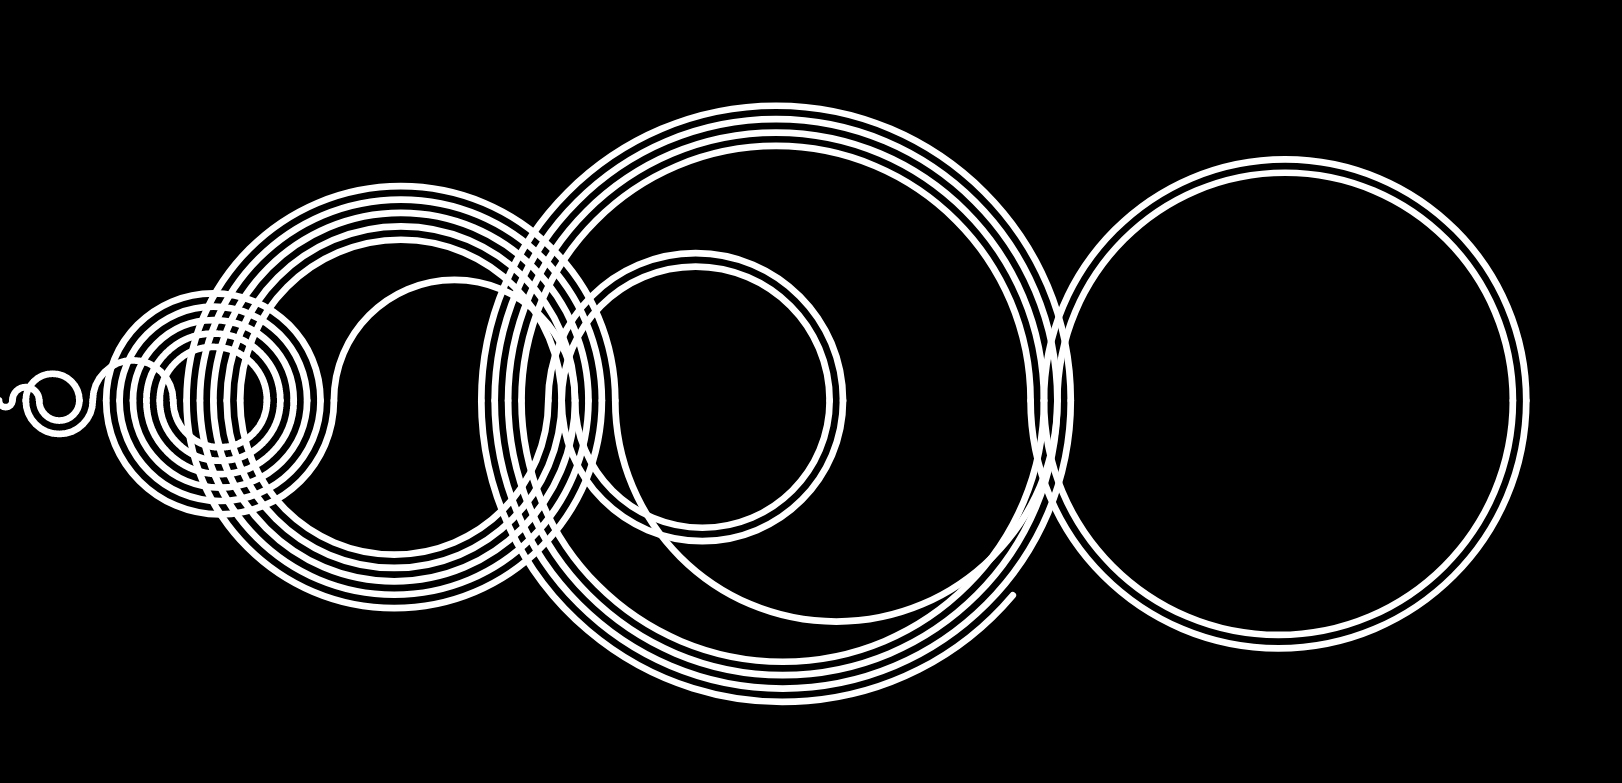
\includegraphics[width=0.7\textwidth]{SoundOfSequences}
\end{figure}

\vfill

Autors del mòdul: Neil J. A. Sloane (dades) i Eric Londaits per a IMAGINARY (Interfície d'usuari).
Text: Daniel Ramos (IMAGINARY).

Referències:
The On-line Encyclopedia of Integer Sequences. \url{www.oeis.org}.

